\section{Introduction}
\par Since its original proposal \citep{Cox1972}, Cox proportional hazards regression has become the most common regression approach for analyzing survival data.  Cox regression utilizes a partial likelihood construction under an assumption of proportional hazards to estimate the regression coefficients without having to specify the underlying baseline hazard.  The ability to avoid choosing a specific parametric distribution for the survival time is very attractive, as time-to-event data are often poorly described by fully parametric models.

%\note{What's with all the \textbackslash par commands?  They don't seem to do anything.}

This semiparametric flexibility, however, comes at a cost. The Cox regression approach can estimate relative risks, but without estimating the baseline hazard, it does not make any predictions concerning the absolute failure time for any given individual.  This poses a challenge to assessing the predictive accuracy of a given Cox regression model.  The challenge is particularly relevant for penalized Cox regression \citep{Tibshirani1997,Fan2002}, as the assessment of predictive accuracy via cross-validation is the standard method for selecting the regularization parameter and deciding upon a model.

\par Standard cross-validation involves dividing the data into $K$ folds, then fitting the model on $K-1$ of those folds (the training set) and assessing prediction accuracy on the remaining fold (the testing set). This process is then repeated, with each fold serving as the testing set exactly once. For Cox regression, the estimated coefficients allow us to quantify the risk for each subject in the training set relative to other members of the training set, but it is not obvious how to use those estimates to quantify the model's accuracy in the testing set.

\par One approach is to simply calculate the partial likelihood based on the observations in the test set as a measure for the model's predictive accuracy.  In doing so, we calculate the risk for each member of the test set relative to other members of the test set.  One drawback to this approach is that it becomes unstable when the size of the the test set is small.  In particular, it cannot be applied to leave-one-out cross-validation (LOOCV), as we must have at least two observations in the test set to compare their risk relative to each other.

%In this paper, we briefly review existing approaches for meeting this challenge, then propose two new methods for carrying out cross-validation in Cox regression models.

%As a semi-parametric model, Cox regression only gives estimations of the $\beta$ coefficients, without estimating the baseline hazard. Hence the interpretation of the Cox model is only valid in a relative sense.

% NOTE: I don't know that we need this paragraph; cross-validation is pretty common.
%One common approach for selecting the tuning parameter $\lambda$ for linear regression and logistic regression is via the K-fold cross validation. The data set would be split into K folds. One fold would be treated as the test set and the other K - 1 folds as the training set. The model would first be built on the training set, then fitted to the test set to obtain cross validation error (CVE).  CVE would be calculated for each candidate $\lambda$, then the one that minimizes cross validated error would be selected.

\par To overcome this drawback, an alternative approach was proposed by \citet{Verweij1993}.  Their approach, which we describe in detail in Section~\ref{Sec:cox-cv-existing}, stabilizes the cross-validated log likelihood, enabling its use even when the number of subjects in each fold is small.  This approach has been widely used and is implemented in R packages such as {\tt glmnet} \citep{glmnet}.  Although this approach fixes the stability issue, we demonstrate here that in practice, it tends to behave conservatively in terms of model selection.

\par In this paper, we propose two alternative ways to carry out cross validation for Cox regression. Instead of applying cross-validation to the partial likelihood directly, we propose applying cross validation to either the linear predictors of the regression model or to the deviance residuals \citep{Therneau1990}. Through simulation studies, we compare these proposed methods with existing cross-validation approaches for LASSO penalized Cox regression in both low- and high-dimensional settings.  %\note{STILL TRUE?? We find that all cross validation approaches tend to be conservative,} \bnote{We should discuss this and the sentence in abstract at our next meeting. They are conservative only in terms of selecting the model that has the best preditive performance; they do not miss selecting variables in the true support}
The linear predictor approach offers the best combination of performance and stability, and we recommend using it for regularization parameter selection in penalized Cox models.  We conclude by applying both proposed and existing approaches to two high dimensional data sets from real studies with time-to-event outcomes.

%%%%%%%%%%%%%
%%%%%%%%%%%%%
\section{Methods}
\label{Sec:methods}
%%%%%%%%%%%%%
%%%%%%%%%%%%%

\par In the Cox model, the hazard function for subject $i$ is given by 
\begin{equation*}
  h_{i}(t) = h_{0}(t) \exp( X_{i}^{T} \beta),
\end{equation*} 
where $h_{0}$ is the baseline hazard and $e^{X_i^{T} \beta}$ is the risk for a subject with covariates $X_i$ relative to that baseline.  The estimation of the coefficients is obtained by maximizing a partial likelihood.  Letting $t_i$ denote the time on study for subject $i$ and $\delta_{i}$ indicate whether or not an event is observed for subject $i$, each subject's individual contribution to that partial likelihood is
\begin{equation}
  \label{eq:cox-pl-subj}
  L_{i}(\beta) = \left \{\frac{\exp ( X_{i}^{T} \beta)}{\sum_{ k \in R(t_{i})}\exp ( X_{k}^{T} \beta)}\right \}^{\delta_{i}},
\end{equation}
where $R(t_{i})$ denotes the set of subjects at risk at time $t_{i}$.  The partial likelihood for the entire sample of $n$ subjects is then given by:
\begin{equation}
  \label{eq:cox-pl-sum}
  L(\beta) =\prod_{i = 1}^{n} L_{i}(\beta).
\end{equation}
Cox regression can be extended by introducing a penalty into the partial likelihood.  In penalized Cox regression, $\beta$ coefficient estimates are obtained by minimizing the objective function
\begin{equation}
  \label{eq:obj}
  Q(\beta) = - \frac{1}{n} \log L(\beta) + P_{\lambda}(\beta),
\end{equation}
where $P_{\lambda}(\beta)$ is a penalty function that depends on a regularization parameter $\lam$.

\par In this paper, we focus upon the LASSO penalty $P_{\lambda}(\beta) = \lambda \sum_{j} |\beta_{j}|$, although the methods we analyze can be used with any penalty as well as with model selection in unpenalized Cox regression (best subset selection). LASSO-penalized cox regression is particularly useful for high dimensional data where the number of covariates $p > n$; for example, in the prediction of overall survival in cancer patients based on genome-wide expression measurements. LASSO estimates yield a sparse model where some coefficients are estimated to be exactly zero. This sparsity pattern changes as we vary $\lam$: at large values of $\lambda$, most or all of the coefficients are 0, but as $\lam$ decreases, more covariates are selected. Selecting $\lambda$ is critical to LASSO estimation in the sense that the model's accuracy suffers if $\lam$ is either too large or too small.

\par Cross-validation is one of the most common methods used to select the appropriate $\lambda$ for penalized regression models. Suppose a data set $D$ of n observations is partitioned into $K$ folds: $D_{1}, D_{2}, \ldots, D_{K}$. For a given $k \in \left\{1,2,\ldots, K\right\}$, let $T_{k} = D - D_{k}$ denote the training set. This manuscript is concerned with the question: how should one use the $kth$ fold $D_{k}$ to measure predictive accuracy based on partial likelihood? In particular, the partial likelihood \eqref{eq:cox-pl-subj} involves a risk set -- which observations should be used to form that risk set?  In the following sections, let $L^{-k}$ denote the partial likelihood built over data in $T_k$, let $L^{k}$ denote the partial likelihood built over data in $D_k$, and $L$ denote the partial likelihood built over the entire data set $D$.  The log partial likelihood is denoted by $\ell$, with $\ell^k$ and $\ell^{-k}$ defined similarly. Finally, let $\hat{\beta}^{-k}$ denote the penalized estimates that are obtained by using $L^{-k}(\beta)$ in \eqref{eq:obj}.

%%%%%%%%%%%%%%%%%%%%
\subsection{Cross validated partial likelihood} 
\label{Sec:cox-cv-existing}
%%%%%%%%%%%%%%%%%%%%

\par A direct approach to measure a model's predictive accuracy in $D_k$ is to evaluate the log partial likelihood at $\hat{\beta}^{-k}$ using the data in $D_k$. Typically, cross-validation error (CVE) is measured by the total deviance across all $K$ folds, which (up to a constant) is given by:
\begin{equation}
  \label{eq:standard}
  \CVE = -2 \sum_{k=1}^{K} \ell^{k}(\hat{\beta}^{-k}).
\end{equation}
%where $\ell^{k}(\hat{\beta}^{-k}) = \sum \limits_{i \in D_{k}} \log L^{k}_{i}(\hat{\beta}^{-k})$.
We refer this approach as \emph{standard cross-validated partial likelihood}. This is implemented in the $\tt{glmnet}$ package as the \verb|"ungrouped"| option. %\note{I added a -2 here so that CVE corresponds to deviance; this is what's done in glmnet/ncvreg}. 

\par The standard approach is by far the most common way of conducting cross-validation for models such as linear regression and logistic regression. However, the standard approach can be problematic for Cox regression in the sense that that there may not be enough observations in $D_k$ to build up the risk set for partial likelihood. For example, the standard approach cannot work with leave-one-out cross-validation, since $\ell_k$ would either be zero or undefined for all folds.

To address this issue, \citet{Verweij1993} proposed an alternative method for cross-validation in Cox models:
\begin{equation}
\label{eq:VVH}
	\CVE = -2\sum_{k = 1}^K \left\{ \ell(\hat{\beta}^{- k})  - \ell^{-k}(\hat{\beta}^{- k}) \right\}. 
\end{equation}
Here, $\ell(\hat{\beta}^{-k})$ is the log partial likelihood evaluated at $\hat{\beta}^{-k}$ using the entire data set $D$ and $\ell^{-k}(\hat{\beta}^{-k})$ is the log partial likelihood evaluated at $\hat{\beta}^{-k}$ on
the training set $T_k$. By avoiding the construction of a partial likelihood on the test set, this approach ensures that the risk set is always sufficiently large and the partial likelihood well-defined.  We refer to this cross-validation method as the Verweij and Van Houwelingen (V\&VH) approach. For many models, such as logistic regression or linear regression, the quantities $\ell(\hat{\beta}^{- k})  - \ell^{-k}(\hat{\beta}^{- k})$ and  $\ell^{k}(\hat{\beta}^{-k})$ are equivalent to each other -- in other words, the standard and V\&VH approaches agree.  However, Verweij and Van Houwelingen's approach is more stable for Cox regression as there is always a large number of observations in the risk sets its calculations are based on.  Since its proposal, the V\&VH approach has been widely implemented as a tool for cross-validation is Cox models.  For example, it is used by the R packages {\tt CoxRidge} \citep{CoxRidge}, {\tt fastcox} \citep{fastcox}, {\tt SGL}\citep{SGL} , {\tt CoxBoost}\citep{CoxBoost}, {\tt mboost}\citep{mboost}, and {\tt glmnet}\citep{glmnet}.  In {\tt glmnet}, it is the default choice for penalized Cox regression and is referred to as the {\tt grouped} option in the package's syntax.

%%%%%%%%%%%%%%%%%%%%
\subsection{Cross Validated Linear Predictors}
\label{Sec:linear-predictor}
%%%%%%%%%%%%%%%%%%%%

\par Both of the methods in Section~\ref{Sec:cox-cv-existing} consist of adding together partial likelihood measures from each fold.  An alternative method is to obtain linear predictors for each fold, then combine these linear predictors to calculate a partial likelihood. We refer to this method as the \emph{cross-validated linear predictors} approach. To be more specific, we would first obtain $\hat{\beta}^{-k}$ from training set $T_{k}$; then the cross-validated linear predictors can be calculated for each observation $i$ from the test set $D_k$:  
\begin{equation}
  \label{eq:cv-lp}
  \hat{\eta}^{cv}_{i} = X_{i}\hat{\beta}^{-k}
\end{equation} 
After repeating this for all K folds, a complete set of cross-validated linear predictors $\hat{\eta}^{cv} = ( \hat{\eta}^{cv}_{1},  \hat{\eta}^{cv}_{2} , ...  \hat{\eta}^{cv}_{n})$ for the whole sample is obtained. A partial likelihood can then be built over this set of linear predictors to evaluate the predictive accuracy of the model: 
	\begin{equation} 
	L(\hat{\eta}^{cv}) = \prod_{i=1}^{n} \frac{\exp (\hat{\eta}^{cv}_{i})}{\sum_{ j \in R(t_{i})}\exp (\hat{\eta}^{cv}_{j})}.
	\end{equation}
We define the cross-validation error evaluated with cross-validated linear predictors to be $$\CVE = - 2 \log L(\hat{\eta}^{cv}).$$
  
\par This idea of obtaining linear predictors over test sets, then constructing the partial likelihood after pooling all linear predictors together is implemented in R package \texttt{ncvreg} \citep{ncvreg}. This idea has also appeared in the cross-validation literature for quantities that cannot be evaluated on only a subset of the data, such as AUC in logistic and Cox regression models \citep{Parker2007,Simon2011a,Subramanian2011}.

%%%%%%%%%%%%%%%%%%%%
\subsection{Cross Validated Deviance Residuals}
%%%%%%%%%%%%%%%%%%%%

The fundamental challenge of conducting cross validation for Cox regression is that the baseline hazard is not estimated from the model. Hence, another approach to cross-validation would be to include an extra step of estimating the baseline hazard and using it to quantify the cross-validation error. The cumulative baseline hazard $\Lambda_0$ is typically estimated via the Nelson-Aalen Estimator \citep{nelson1969, aalen1978}:
\begin{equation}
  \hat{\Lambda}_{0}(t) = \sum_{t_j \leq t}\frac{\text{number of failures at time } t_j}{\text{number at risk right before time }t_j}.
\end{equation}
\bnote{I write out the $t^{-}_j$ definition directly into the fomula so that we don't need to define $t^{-}_j$ separately.}
The Cox model implies the following relationship between the baseline cumulative hazard and the cumulative hazard for individual $i$:
\begin{equation}
  \hat{\Lambda}_{i}(t) =  \hat{\Lambda}_{0}(t)\exp(X_i\hat\beta).
\end{equation}

The baseline hazard could be incorporated into cross-validation in a variety of ways.  Here, we consider the following approach: for fold $k$, we obtain $\hat{\beta}^{-k}$ from the training set $T_k$ and then for each $i$ in the test set $D_k$, 
\begin{equation}
 \label{eq:cv-bhz}
  \hat{\Lambda}^{cv}_{i}(t) =  \hat{\Lambda}_{0}(t)\exp(X_i\hat\beta^{-k}).
\end{equation}
Note that this uses an estimate of the baseline hazard coming from the full data under the null model, but cross-validation has been applied to the estimation of the regression coefficients $\hat{\beta}$; we will discuss the rationale for this estimator shortly.

A natural candidate for incorporating the cumulative hazard into a loss function is the deviance residual, a normalized form of the Martingale residual \citep{Therneau1990}. First proposed for model diagnostics, deviance residuals have also been occasionally used as a predictive accuracy measure \citep{Therneau2018}.  Given \eqref{eq:cv-bhz}, we can first obtain the cross-validated Martingale residual: 
\begin{equation}
  \hat{M^{cv}_{i}} = \delta_{i} - \hat{\Lambda}_{0}(t_{i})\exp(X_i\hat\beta^{-k}).
\end{equation}
The cross-validated deviance residuals can then be derived from the Martingale residuals: 
\begin{equation} 
  d_{i} = \text{sgn}(\hat{M}^{cv}_{i})\sqrt{-2(\hat{M}^{cv}_{i} + \delta_{i}\log(\delta_{i} - \hat{M}^{cv}_{i}))}.
\end{equation}
The sum of squared cross-validated deviance residuals, $\sum_{i}\hat{d}_{i}^2$ are used as the cross validated error as an analogy to the residual sums of square for linear regression. We refer to this method as the \emph{cross-validated deviance residuals} approach.

The baseline hazard estimate we describe here differs from the one typically used in constructing deviance residuals \citep{Therneau1990}. Instead of the Nelson-Aalen estimator, deviance residuals are typically calculated based on a baseline hazard estimate that has been adjusted for the covariates in the model such as the one described in \citet{breslow1972}. In the context of cross-validation, however, this approach is problematic. Deviance residuals measure the difference between the fitted model and a saturated model; in Cox regression, this saturated model depends on the baseline hazard. Thus, a covariate-adjusted baseline hazard would mean that each fold is compared to a different saturated model. For this reason, we consider it important that the baseline hazard remains constant across folds when calculating cross-validated deviance residuals; this intuition is borne out by simulations involving various other approaches \note{supplement? otherwise, this sentence is a little tricky}\bnote{sure}.  Note that this is not the case for the Brier Score or Kullback Leibler Score (described in Section~\ref{Sec:accuracy}), which involve absolute loss functions, not comparisons with a saturated model.

%A more straightforward way to compute the cross-validated deviance residuals is to estimate the baseline hazard using $T_k$, leaving $D_k$ as out-of-sample observations to calculate the residuals. There are two major issues with this approach. First, it is possible that some events in $D_k$ occurred after the last event in $T_k$. In this case, the survival function would drop to 0. Secondly, there is a numeric challenge for computing the term $log(\hat{\Lambda}_{0}(t_{i})e^{\hat{\eta}_{i}})$ in deviance residuals. Since the baseline hazard function is a step function from 0, the cumulative hazard $\hat{\Lambda}_{0}$ at the first time point from 0 is always 0. For whichever $D_k$ that contains the first time point, $log(\hat{\Lambda}_{0}(t_{i})e^{\hat{\eta}_{i}})$ would be negative infinity for that observation and lead to a numeric issue. To solve the first issue, events that occur later than the last event in $T_k$ should be censored. To solve the second issue, the step function of the baseline hazard needs to be smoothed. Both issues do not exist when the baseline hazard is built over the cross-validated linear predictors using all samples. \note{this paragraph may be optional, and can also be moved to discussion}

\begin{figure}
  \centering
  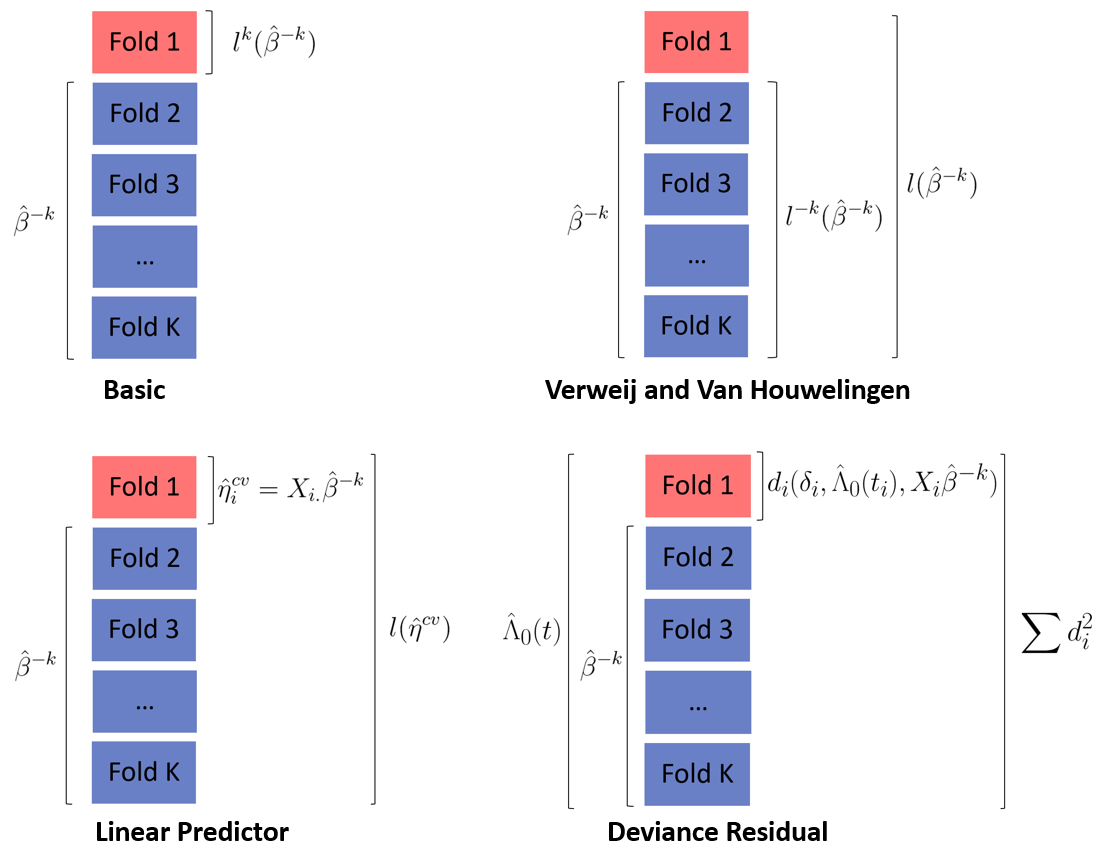
\includegraphics[height= 12cm ]{./manuscript_figure/figure_1_new.png}
  \caption{Illustration of K-fold Cross Validation Methods for Cox Regression}
\end{figure}	

%%%%%%%%%%%%%%%%%%%%
%%%%%%%%%%%%%%%%%%%%
\section{Simulation Studies}
%%%%%%%%%%%%%%%%%%%%
%%%%%%%%%%%%%%%%%%%%

Simulation studies were conducted to compare how the methods described in Section~\ref{Sec:methods} behave relative to each other in selecting the tuning parameter $\lambda$ and the corresponding model for LASSO penalized regression. For these simulation studies, the covariate matrix $X$, consisting of $n$ observations and $p$ covariates, was generated from independent $\text{Normal}(0, 1)$ samples. Given $X$ and a coefficient vector $\beta$, survival times were generated from exponential distribution with rate parameter $\exp(X\beta)$. Censoring status indicators were drawn independently from the binomial distribution. All simulations were implemented in R \citep{R}. We varied the sample size, dimension, censoring percentage and signal strength of the simulated data sets to examine how these factors affect the performance of cross-validation.
   
%%%%%%%%%%%%%%%%%%%%%%%%%%%%%%%%
\subsection {Simulations Comparing Predictive Accuracy}
\label{Sec:accuracy}
%%%%%%%%%%%%%%%%%%%%%%%%%%%%%%%%

Our first simulation study concerns the accuracy of the cross-validation approaches introduces in Section~\ref{Sec:methods}.  Accuracy was assesed via several criteria.

Estimation accuracy was measured using the mean squared error of the coefficients ($\MSE$). Suppose $\hat{\beta}(\lambda)$ is the set of coefficients estimated by a cox model with LASSO penalty at $\lambda$. Mean squared error $MSE$ is defined to be 
%\bnote{
\begin{equation}
E\| \hat{\beta}(\lambda) - \beta \| ^2.
\end{equation}
%}
%\note{this is the equation for a scalar MSE, not a vector}

Throughout, we communicate the estimation accuracy in terms of relative MSE, as compared to the oracle model.  For each generated data set, an oracle model was fit using Cox regression only including the variables with non-zero coefficients. Letting $\hat{\beta}^{oracle}$ denote the resulting estimates, the relative MSE, on the log scale, is given by
\begin{equation}
\log\left\{ \frac{\MSE(\hat{\beta}(\lambda^{\text{cv}}))}{\MSE(\hat{\beta}^{\text{oracle}})} \right\},
\end{equation}
where $\lambda^{cv}$ denotes the value of $\lambda$ selected by cross-validation. MSE is estimated by avevaring over N replications respectively for $\hat{\beta}(\lambda^{cv})$ and $\hat{\beta}^{oracle}$. The ratio is taken afterwards. The $\log$ is taken to correct for skewness. %\note{I'm not sure why this is a note; shouldn't you rewrite the sentence?}

\par We also measure the predictive accuracy via the mean squared prediction error, or Brier score \citep{VanHouwelingen2011}. Let $\hat{S}(t_0|\lambda,x)$ denote the predicted probability for an individual with covariates $x$ to survive beyond time $t_0$, and let $y = \mathbb{1}\left\{ t > t_{0}\right\}$ indicate whether the individual actually survived beyond time $t_0$. Then the Brier score is defined to be
\begin{equation}
\text{Brier}(y, \hat{S}(t_0|\lambda,x)) = (y - \hat{S}(t_0|\lambda,x))^2.
\end{equation}
In our simulation study, for each data set, we generated another independent data set with 1000 uncensored observations. We computed Brier scores for all of the cross-validation methods for all individuals in this test set, setting $t_0$ to the median survival time.

\par The third measure we used is the Kullback-Leibler score, which measures the log-likelihood of the prediction model evaluated at the observations \citep{VanHouwelingen2011}. With the same notation defined in the previous paragraph, the Kullback-Leibler score is defined to be
\begin{equation}
	\text{KL}(y, \hat{S}(t_0|\lambda,x)) = -\left\{ y\log(\hat{S}(t_0|\lambda,x) + (1 - y)\log(1 - \hat{S}(t_0|\lambda,x)) \right\}.
\end{equation}
As for the Brier score, KL scores were computed for all CV approaches at the median survival time.  Results were then averaged over the N replications. For both Brier and KL scores, a score represents smaller prediction error, thus indicating better prediction accuracy.

\par The final metric we included in our study was Harrell's C Index \citep{HarrellJr1984}. The C Index is a rank-based statistic that measures the concordance between the linear predictor of the selected model and the observed outcome. Suppose we arbitrarily select two individuals; if the individual with the higher predicted risk also died first, then this would be considered as a concordant pair. The C Index considers all possible such pairs and estimates of proportion of those pairs that are concordant. A C Index of 0.5 means the prediction is no better than flipping a coin and C Index of 1 means perfect concordance. We computed Harrell's C Index using the independent test set of 1000 individuals described above.

 For each simulated data set, the covariate matrix has $n = 120$ observations and $p = 1000$ covariates. The covariate vector $\beta$ is assumed to be sparse, with $\beta_j = 0$ for $j \in \{11,12,..,1000\}$ and $\beta_j = s$ for $j \in \{1,2, ..., 10 \}$, where $s$ is a prespecified constant that parameterizes the signal strength in the simulated data set. In the first simulation study, we varied $s$ from 0.4 to 0.9. The survival outcomes have 10$\%$ expected censoring. For each of the four methods described in Section~\ref{Sec:methods}, 10-fold cross-validation was implemented. $N = 200$ replications were used for each scenario.

\begin{figure}[ht]
  \centering
  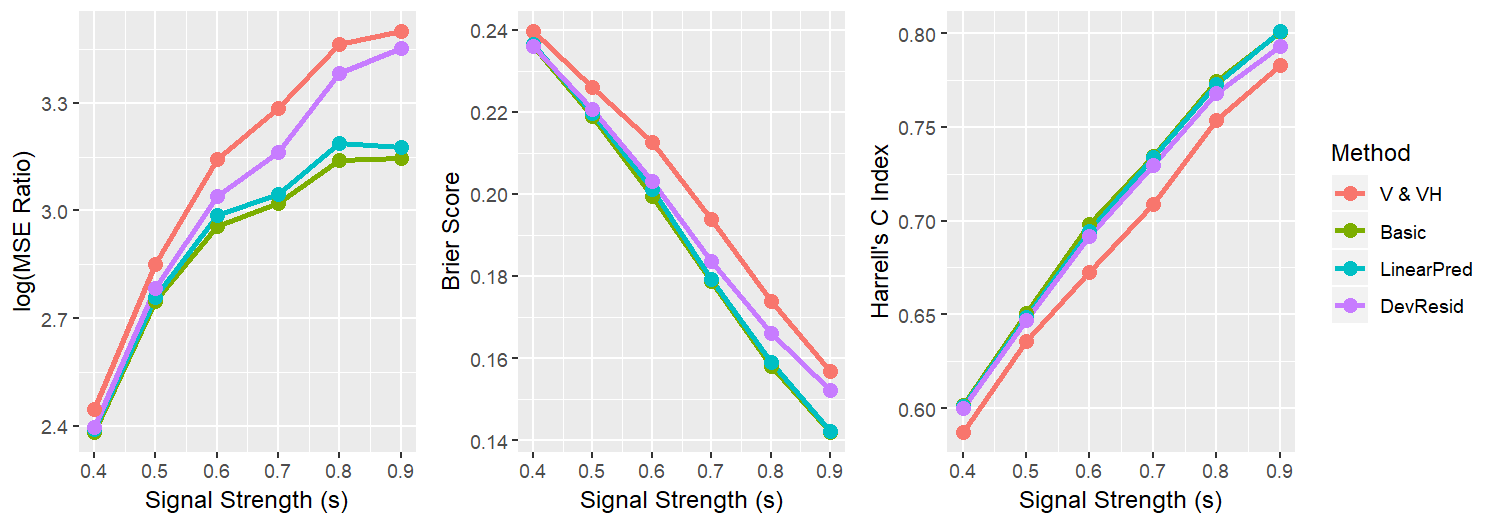
\includegraphics[height= 7cm ]{./manuscript_figure/figure_2_new.png}
  \caption{\label{Fig:mse-brier-c} Simulation comparing 4 CV methods. The horizontal axis in all three plots is $s$, which represents the signal strength in the data. The value of $s$ is varied from 0.4 to 0.9.  $\log(\text{MSE ratio})$, relative to the oracle modle is plotted in the left panel. Out-of-sample Brier scores are plotted in the middle. Out-of-sample Harrell's C index is plotted in the right panel. For each simulated data set, n = 120, p = 1000. Expected censoring percentage is 10$\%$. \note{I really think the x axis should be Signal (s) or Signal strength (s)}}
\end{figure}	

%The left panel compares the $\lambda$ selected by different methods. Verweij and Van Houwelingen's cross-validated partial likelihood approach, which is currently most widely used approach, consistently selects $\lambda$s that are greater than the optimal one.  Greater $\lambda$ leads to greater penalties and fewer non-zero variables, hence Verweij and Van Houwelingen's approach is conservative in terms of selecting variables. While the proposed cross-validated Deviance residual has very close performance as Verweij and Van Houwelingen's approach, the standard cross-validated log likelihood and the cross-validated linear predictor were more liberal than the other two methods. In general, all four methods tends to act conservatively and selects smaller models. 

\par Figure~\ref{Fig:mse-brier-c} illustrates the results of this simulation study. In each panel, the horizontal axis is the magnitude of the non-zero $\beta$ coefficients.  For all four metrics, the overall pattern is the same (KL scores not shown in Figure~\ref{Fig:mse-brier-c} due to space constraints, but they were very similar to Brier scores).  Although the four cross-validation methods performed relatively similarly, the standard and linear predictor approaches had the best performance across all metrics: lower MSE, better Brier scores, and higher concordance.
 
\begin{table}[htb]

\setlength{\tabcolsep}{3pt}

\caption{\label{Tab:sim} Simulation comparing four cross-validation methods with varying dimension and signal strength}
\centering
\begin{tabular}[t]{cccccccccc}
\toprule
 n& p& $\#$ Non-Zero & Signal & Method & $\lambda$ & log(MSE Ratio) &Brier Score & Kullback Leibler & C Index\\
\midrule
150 & 50 & 5 & weak & V VH  & 0.098 (0.030) & 1.561 (0.851) & 0.245 (0.014) & 0.685 (0.030) & 0.610 (0.035) \\
    &    &   &     & Standard  & 0.088 (0.025) & 1.531 (0.838) & 0.244 (0.013) & 0.683 (0.029) & 0.614 (0.029) \\
    &    &   &     & LinearPred  & 0.092 (0.029) & 1.543 (0.846) & 0.245 (0.014) & 0.684 (0.030) & 0.612 (0.034) \\
    &    &   &     & DevResid  & 0.098 (0.029) & 1.547 (0.848) & 0.245 (0.014) & 0.684 (0.030) & 0.611 (0.035) \\
\addlinespace
150 & 50 & 5 & strong & V VH  & 0.071 (0.010) & 1.586 (0.989) & 0.176 (0.011) & 0.526 (0.027) & 0.750 (0.012) \\
    &    &   &     & Standard  & 0.066 (0.011) & 1.544 (0.971) & 0.176 (0.011) & 0.526 (0.028) & 0.749 (0.013) \\
    &    &   &     & LinearPred  & 0.067 (0.010) & 1.540 (0.981) & 0.176 (0.011) & 0.525 (0.028) & 0.750 (0.012) \\
    &    &   &     & DevResid  & 0.094 (0.011) & 1.995 (0.841) & 0.181 (0.011) & 0.539 (0.026) & 0.751 (0.013) \\
\addlinespace
400 & 10000 & 20 & weak & V VH  & 0.126 (0.019) & 2.958 (0.416) & 0.251 (0.012) & 0.696 (0.026) & 0.589 (0.044) \\
    &    &   &     & Standard  & 0.103 (0.022) & 2.880 (0.437) & 0.244 (0.015) & 0.680 (0.031) & 0.603 (0.039) \\
    &    &   &     & LinearPred  & 0.105 (0.023) & 2.886 (0.437) & 0.244 (0.015) & 0.681 (0.031) & 0.602 (0.039) \\
    &    &   &     & DevResid  & 0.107 (0.022) & 2.895 (0.433) & 0.245 (0.014) & 0.683 (0.03) & 0.602 (0.039) \\
\addlinespace
400 & 10000 & 20 & strong & V VH  & 0.084 (0.012) & 3.799 (0.548) & 0.176 (0.03) & 0.528 (0.069) & 0.763 (0.048) \\
    &    &   &     & Standard  & 0.059 (0.007) & 3.455 (0.578) & 0.154 (0.019) & 0.468 (0.049) & 0.780 (0.031) \\
    &    &   &     & LinearPred  & 0.060 (0.007) & 3.479 (0.574) & 0.155 (0.019) & 0.470 (0.049) & 0.780 (0.030) \\
    &    &   &     & DevResid  & 0.076 (0.018) & 3.708 (0.518) & 0.166 (0.024) & 0.502 (0.057) & 0.772 (0.049) \\
\bottomrule
\end{tabular}
\end{table}

Table~\ref{Tab:sim} displays the results of additional simulations carried out as we varied the dimension of the data set along with the signal strength.  Specifically, we examined the following settings: low dimension (p = 50) with weak signal, low dimension with strong signal, high dimension (p = 10000) with weak signal, and high dimension with strong signal. In all settings, the censoring rate was 30\%.

As in Figure~\ref{Fig:mse-brier-c}, the standard and linear predictor approaches outperform the deviance residual and V\&VH approaches.  The improvement is particularly noticeable in the most difficult setting: high-dimensional data with weak signal.  Table~\ref{Tab:sim} also provides some insight into why the deviance residual and V\&VH approaches perform poorly relative to standard CV and the linear predictor approach: they act conservatively, consistently choosing larger $\lam$ values and selecting fewer variables. %\note{if we're going to say something about ``selecting fewer variables'', should Table 1 include the average model size?} \bnote{I'm afraid that the average model size would be confusing to the readers. The most conversative model would have the smallest model size, and would be closest to the true model size}

\subsection {Stability}
\label{Sec:stability}
  \bnote{still working on a new simulation}
\par In this section, we present a small simulation study to illustrate the numerical stability issues faced by standard cross-validation in the partial likelihood setting.  The standard approach is both straightforward and enjoys very good predictive accuracy, as seen in Section~\ref{Sec:accuracy}. The main drawback to its widespread use is that the number of uncensored observations in the test set may be insufficient to construct a well-defined partial likelihood, leaving the overall estimate of cross-validation error undefined as well.

To illustrate how common this problem is, and what factors it depends on, we conducted a simulation study varying the number of folds and censoring rate. Throughout we fixed the number of observations at $n = 100$. When varying the censoring rate, we fixed the number of folds at $K = 10$; when varying the number of folds, we fixed the censoring rate at 10\%. We generated 200 independent data sets according to the mechanism described in Section~\ref{Sec:accuracy} and recorded whether or not standard cross-validation was able to be carried out (i.e., whether the partial likelihood was well-defined for all folds).

\note{did we make an effort to balance censoring across folds here?  we should comment on this}

\note{also, hmm, censoring rate isn't actually fixed at, say, 30\%...eh, maybe it's OK}

\par As illustrated in Figure~\ref{Fig:stability}, at $n=100$ the standard approach can be problematic even at fairly modest censoring rates.  For example, standard CV cannot be used with over 25\% of data sets when half of all observations are censored.  Furthermore, even if the censoring rate is just 10\%, standard CV strongly limits the number of folds that can be included in the cross-validation process, becoming very unstable when the number of folds exceeds 10.

\begin{figure}[h]
  \centering
  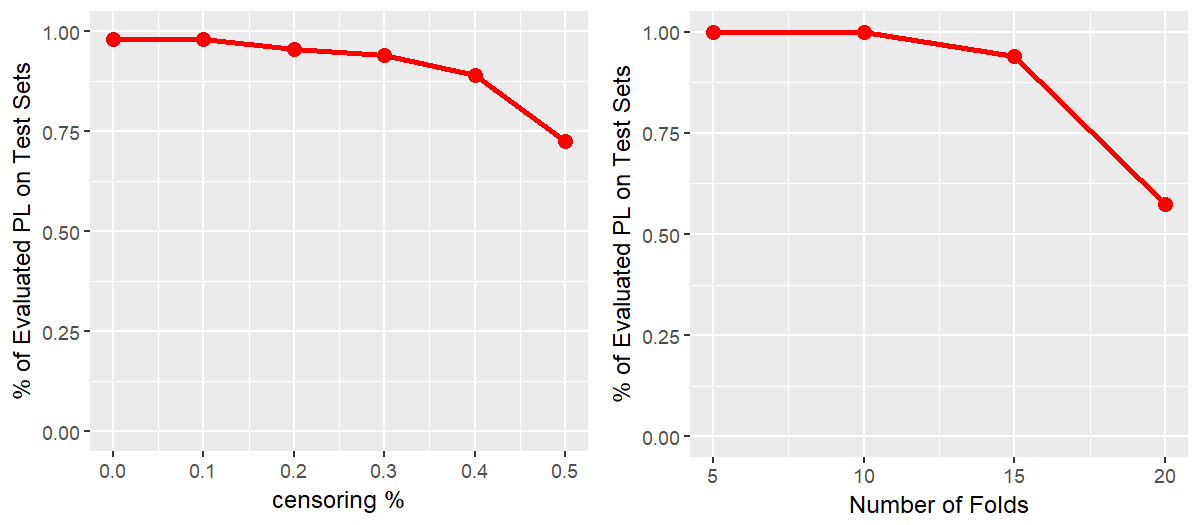
\includegraphics[height= 7cm ]{./figures/figure_3_new.png}
  \caption{\label{Fig:stability}Comparing Stability \note{This plot needs better y axis labels and caption; also, these are not percents.}}
\end{figure}	

\subsection {Leave-One-Out Cross Validation}
\label{Sec:loocv}

\bnote{Simulation Updated, still need to work on writing}
As discussed earlier, standard cross-validation cannot be used to carry out leave-one-out cross validation (LOOCV) for Cox regression models.  The three other approaches (V\&VH, linear predictor, and deviance residual), however, are not subject to the stability issues described in Section~\ref{Sec:stability}, and can be used to implement LOOCV.  Here, we compare these three approaches for carrying out LOOCV, and also compare LOOCV to 10-fold CV.

For this study, we conducted both 10-fold CV and LOOCV for the V\&VH, linear predictor, and deviance residual approach, with standard 10-fold cross-validation used as a baseline for comparison.  These results are shown in Figure~\ref{Fig:loocv}. \note{FYI, never write \texttt{Figure 4}; always use \texttt{\textbackslash ref}} For all three methods, LOOCV selected models with a smaller MSE than 10-fold CV. For the V\&VH and deviance residual approaches, however, LOOCV was still was inferior to standard 10-fold CV.  As described in Section~\ref{Sec:stability}, these approaches tend to be conservative, selecting a larger-than-optimal value of the regularization parameter; LOOCV helps with this problem, but does not alleviate it entirely.

For the linear predictor approach, on the other hand, \ldots \note{we need to talk about the linear predictor approach too!}

\begin{figure}[h]
  \centering
  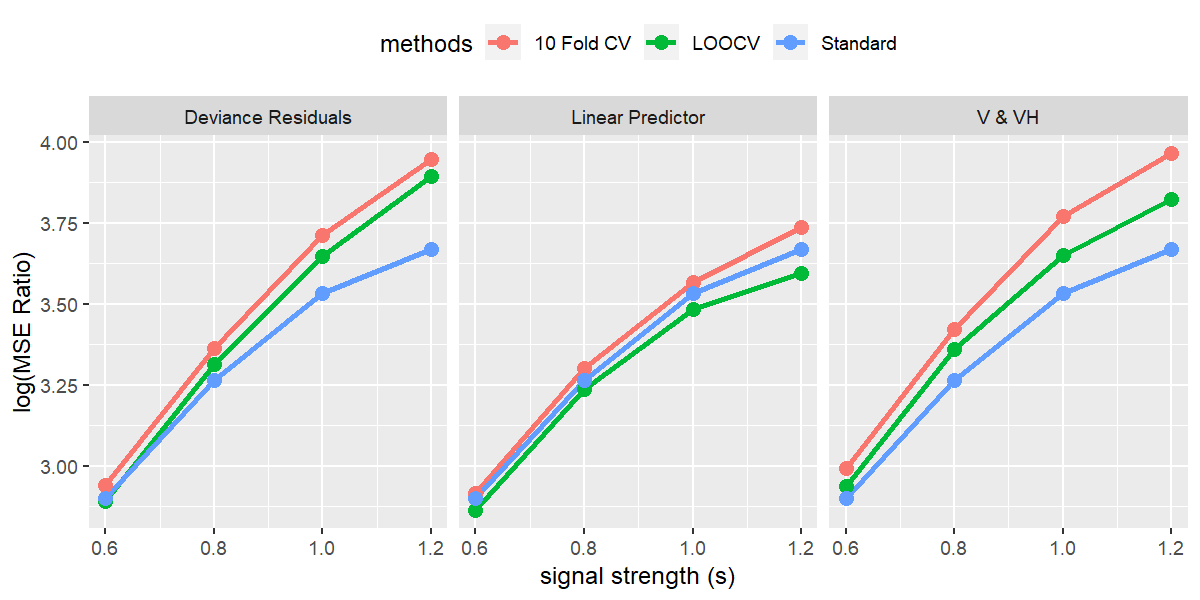
\includegraphics[height= 8cm ]{./manuscript_figure/figure_4.png}
  \caption{\label{Fig:loocv}LOOCV\note{Needs a better caption; also, should y-axis be log mse ratio?}}
\end{figure}	

\subsection {Cross-Validated C Index}

\par All of the cross-validation approaches described in Section~\ref{Sec:methods} use the Cox partial likelihood, in one way or another, as the criterion upon which model selection is based.  In this section, we compare these likelihood-based approaches against an alternative approach of cross validation using concordance, also known as the cross-validated AUC (CV-AUC).  This is a widely used approach to cross-validation with time-to-event outcomes, particularly for machine learning models that are not likelihood-based \citep{Subramanian2011,Simon2011a}. This approach typically proceeds by constructing cross-validated linear predictors, as in Section~\ref{Sec:linear-predictor}, but then using those predictors to calculate concordance as opposed to partial likelihood.

\par We conducted simulations in both low dimensional ($p = 50$) and high dimensional ($p = 1000$) settings, varying the signal in the data \note{as in Section 3.1?} \note{is $n=100$ here?}. Results of the simulations are illustrated in Figure 5 \note{make this into a reference}.  We used the linear predictor approach (CV-LP) here as the representative approach for likelihood-based cross-validation.

\begin{figure}[h]
  \centering
  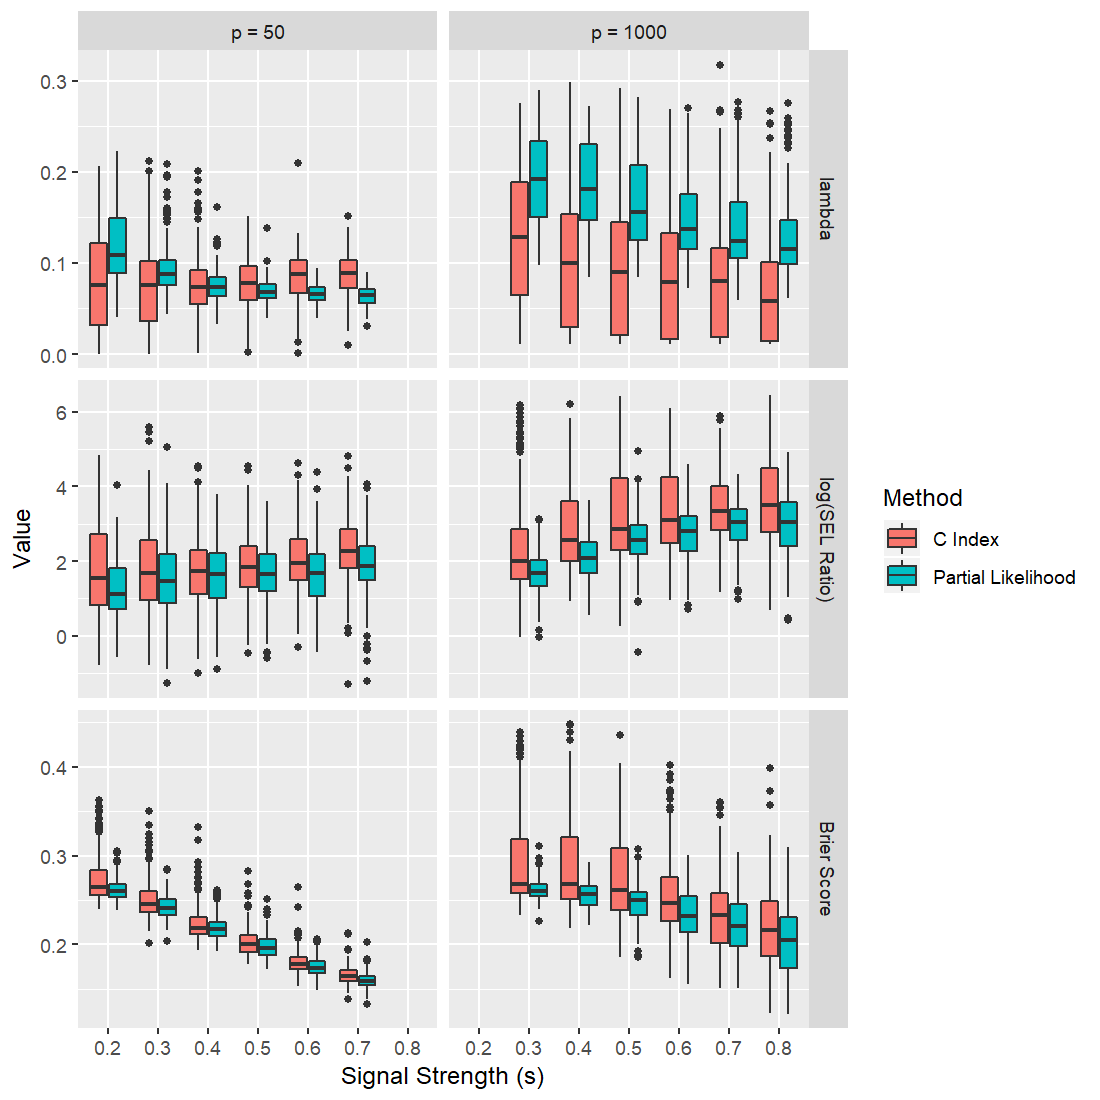
\includegraphics[height= 15cm ]{./manuscript_figure/figure_auc.png}
  \caption{\bnote{caption edited}Comparing Partial Likelihood and C Index both built from Cross-validated Linear Predictors. The horizontal axis represents the strength of signal $s$ in the data. The left figures are under the low dimension scenarios where p = 50 and n = 150. The right figures are under the high dimension scenarios where p = 1000 and n = 120. The expected percentages of censoring for both scenarios are 30 $\%$. The top row are box plots of the selected tuning parameter$\lambda$. The mid row plots the $\log(\text{SE Ratio})$ \bnote{(it just occured to me, this may not exactly be the log of MSE ratio. because to get MSE, we need to take average over all replications. But this figure is plotting each replication...)}, relative to the oracle model. The bottom row plots the Brier Scores. }
\end{figure}

Several observations can be drawn from Figure~\ref{5}.  First, likelihood-based CV tends to select more accurate models, as judged by both mean squared error and Brier score.  Second, likelihood-based CV is also more stable than the AUC-based CV, in the sense that it tends to select a narrower range of models, with more consistent performance, than CV-AUC.  Lastly, CV-AUC is consistently more liberal than likelihood-based CV, selecting models with smaller values of the regularization parameter $\lam$, and therefore preferring models with larger coefficient values and more nonzero coefficients.

\section{Application to Real Data}

\par In this section, we apply the cross validation methods described in Section~\ref{Sec:methods} to data from a study of gene expression and survival in patients with lung cancer. \citet{shedden2008gene} conducted a large, retrospective study to validate prognostic gene expression signatures as predictors of overall survival in lung cancer patients.
They gathered expression profiles of \textit{22,283} genes for \textit{442} \note{is there some reason 442 is in italics? other numbers aren't} non-small-cell lung cancer (NSCLC) patients along with a number of clinical variables such as stage, age and gender. \note{Did you only adjust for stage, age, and gender, or did you adjust for smoking, etc., as well?  If not, maybe take out ``such as'', which implies that there are other variables you're not mentioning.} About 50\% of the patients died during the course of the study (236 events), with the rest censored. The clinical variables stage, age and gender were known to have a larger prognostic impact, thus they were fitted in the model without penalization. Cross-validation was again used for the selection of the penalty term, which selects the gene expressions that are associated with patients' overall survival. The results of the analysis are also listed in Table 3.

\par How the CV methods perform on real data reflects what is shown in simulation studies. The standard CVE is the most liberal approach. Deviance Residual and Verweij and Van Houwelingen's CVE approaches were both really conversative, while the standard approach was the second liberal to standard CVE. In Figure 5, the Cross Validated Error is rescaled and plotted for all four methods. A $\lambda$ will be selected when CVE curve reaches its lower point. The blue line, which represents the linear predictor approach, has more curvature near its lowest point. It is easier to pick out the minimum point for this blue curve. Hence this approach is better at picking out signals than the other three approaches. For Verweij and Van Houwelingen's cross-validated partial likelihood, there's almost no signal there.

\begin{figure}[h]
    \centering
		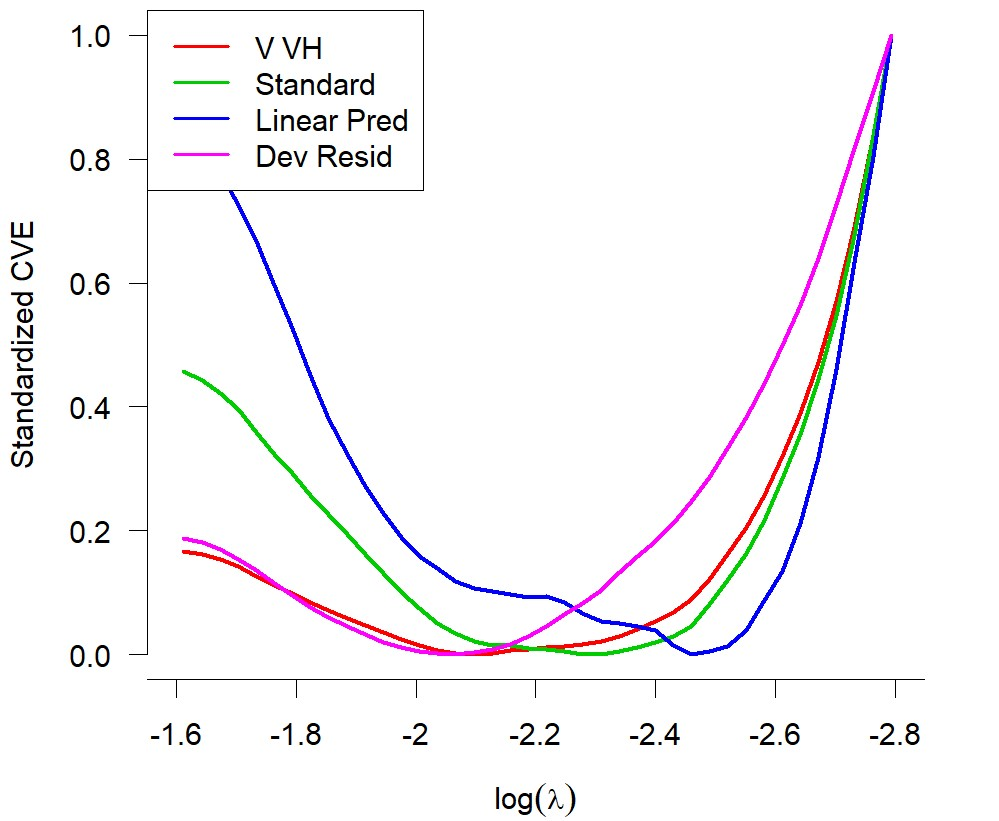
\includegraphics[height= 8cm ]{./figures/shedden.jpg}
    \caption{Comparing Cross-Validated Error for Different Methods on Real Data Sets}
\end{figure}	

\begin{table}[h]
\centering
\caption{Application to Real Data Sets}
\label{my-label}
\begin{tabular}{lccccc}
\toprule
						& $\lambda$ & log($\lambda$) & CV AUC & Brier Score \\ 
						\cline{2-5} \\ 
						V $\&$ VH& 0.123 & -2.097 & 0.640 & 0.246\\
						standard & 0.102 & -2.278 & 0.643& 0.239\\
						Linear Pred &0.085 & -2.460 & 0.651&  0.227\\
						Dev Resid & 0.127& -2.066 & 0.639& 0.246\\ 
						\bottomrule
\end{tabular}
\end{table}

\section{Discussion}

\par Four methods of conducting cross-validation for Cox Regression were compared through simulation studies in terms of their predictive accuracy. All cross-validation methods tend to select the more conservative model: with greater value of $\lambda$, and fewer variables selected into the model. Despite of the stability issue, the standard approach is the most liberal one across all scenarios and yield the least MSE. The proposed linear predictor approach performs closely to the standard approach. Under LOOCV, the linear predictor approach out-performs the standardstandard approach. Both Verweij and Van Houwelingen's approach and the proposed Deviance Residual approach perform conservatively, hence not recommended for use in practice. Results from real data application reflects results from the simulation studies.

% Discussion on Deviance Residual

%\par While the Deviance Residual approach has a reasonable performance in scenarios where dimension is high, it tends to act more conservatively than all the other three approaches in general. As is noted by Therneau et al, the sums of squared martingale residuals and deviance residuals do not necessary reflect how good the model fit is \citep{Therneau2000modeling}. The difficulty of estimating the baseline hazard seems to play an important role. A series of simulations were thus designed to study how baseline hazard estimation affects the deviance residuals' performance as a measurement for model fit. 

%\par In the following simulation studies, the defined optimal $\lambda$ and the $\lambda$ selected by the Linear Predictor approach were used as benchmarks. Various sample sizes and dimensions were varied. The survival outcomes were generated both from exponential distribution and Weibull distribution. Six different approaches were compared in terms of baseline hazard estimation and their impact on sums of squared deviance residuals. Two non-parametric approaches, Kalbfleisch and Prentices' estimator and Breslow's estimator, were used first for estimating the cumulative hazard baseline \citep{Kalbfleisch2011} \citep{breslow1972}.  As is presented in column 3 and column 5 in Table 2, the sum of squared deviance residuals computed based on both approaches are all very conservative compared to the optimal $\lambda$. Their performance is extremely bad when n is large and p is small. 

%\par Since both of the non-parameteric estimations seemed to perform well at early time points but poorly later, a weighted approach was then applied to emphasize earlier time points. Weights are assigned proportional to number of subjects at risk, making earlier time points weighted more than later time points. Results of these two approahces are presented in column 4 and 6 in Table 2. The attempt to improve the non-parameteric estimations via weighting does not seem to improve the selection too much. 

%\par In the next step,  the non-parametric baseline hazard estimation was replaced by the exact baseline hazard that was used to generate the outcome. Results were listed in the seventh column in Table 2. When the baseline was known, the performance of sum of squared deviance residuals actually performed really close to the optimal $\lambda$. This simulation suggests that when the baseline hazard was accurately estimated, then the sum of squared deviance residuals gave really good measures for the model fit.

%\par In the last step, we replaced the non-parametric baseline hazard estimation with a parametric approach, where we assume the baseline hazard to follow an exponential distribution. We derived the estimation for baseline hazard by maximum likelihood approach conditioned on covariates: $\hat{\lambda}_{0} = \frac{\sum d_{i}}{\sum t_{i}e^{\eta_{i}}}$. The results are listed in the eighth column in Table 2. When this estimation was used for data that were generated from exponential distribution, its performance was as well as when the exact baseline was specified. When it was fitted to data that were generated from the Weibull distribution, that is when the model is misspecified, then its performance was even worse than the non-parametric approaches.

%\par Hence, getting accurate estimation of the baseline hazard is crucial to whether or not the sum of squared deviance residuals can be a good measurement for model fit.

%\begin{table}[h]
%	\small
%	\caption{Average of Selected $\lambda$ with Different Baseline Estimation for Deviance Residuals}
	%\centering
	%\begin{tabular}{lllllllll}
	%\hline
	%\\[-0.75em]
    %& Optimal & Linear Pred & KP & KP & Breslow & Breslow & Exact & Exp\\ 
    %&  & & & weighted & & weighted & & \\ \cline{2 - 9} 
	%\textbf{True Baseline: $Exponential(1)$} &&&&&&&&\\
	%n = 100, p = 10, non-zero $\beta$: 2 & 0.0461 & 0.0665 & 0.1986 & 0.1970 & 0.1908 & 0.1975 & 0.0540 & 0.0539 \\
	%n = 100, p = 100, non-zero $\beta$: 20 &0.0555 & 0.1841 & 0.2359 & 0.2201 & 0.2146 & 0.2244 & 0.0805 & 0.0985 \\
	%n = 100, p = 1000, non-zero $\beta$: 20 & 0.0268 & 0.0505 & 0.0948 & 0.0798 & 0.0867 & 0.0809 & 0.0288 & 0.0270 \\
	%\textbf{True Baseline:} $Weibull$ &&&&&&&& \\
 	%n = 100, p = 10, non-zero $\beta$: 2 & 0.0476 & 0.0710 & 0.2004 & 0.1969 & 0.1907 & 0.1907 & N/A & 0.2330 \\ 
	%\hline
%\end{tabular}
%\end{table}


\section{Appendix}

\begin{figure}[h]
	\centering
	\begin{minipage}[t]{10cm}
	\begin{algorithm}[H]
	\caption{Standard Method}
	\par \For{k in 1 to K } 
	{
		 Fit Cox Regression on $T_{k}$: Obtain model estimates $\hat{\beta}^{-k}$\;
		 Evaluate the partial likelihood of $\hat{\beta}^{-k}$ on $D_{k}$: $l^{k}(\hat{\beta}^{-k})$\;		
	} 
	
	\par $ CVE_{st} = - \sum_{k = 1}^{K} l^{k}(\hat{\beta}^{-k})$
 	\end{algorithm}

	\begin{algorithm}[H]
  	 \caption{Verweij and Van Houwelingen's Method}
	\par \For{k in 1 to K } 
	{
		 Fit Cox Regression on $T_{k}$:  Obtain model estimates $\hat{\beta}^{-k}$\;
		 Evaluate the partial likelihood of $\hat{\beta}^{-k}$ on $T_{k}$: $l^{-k}(\hat{\beta}^{-k})$\;
		 Evaluate the partial likelihood of $\hat{\beta}^{-k}$ on $D$: $l(\hat{\beta}^{-k})$\;
		 Take the difference: $ l(\hat{\beta}^{-k}) - l^{-k}(\hat{\beta}^{-k}) $\;
	} 

	\par $ CVE_{vvh} = - \sum_{k = 1}^{K} \left\{ l(\hat{\beta}^{-k}) - l^{-k}(\hat{\beta}^{-k}) \right\}$
	\end{algorithm}

	\begin{algorithm}[H]
    	\caption{Cross-Validated Linear Predictors}
	\par \For{k in 1 to K } 
	{
		 Fit Cox Regression on $T_{k}$:  Obtain model estimates $\hat{\beta}^{-k}$\;
		$\forall$ $ i$ subject in $D_k$: $\hat{\eta}_{i}^{-} = X_{i}\hat{\beta}^{-k}$\;
	} 

	\par $ CVE_{lp} = - l(\hat{\eta}^{-})$
	\end{algorithm}
	
	\begin{algorithm}[H]
   	\caption{Sums of Squared Deviance Residuals}
	\par \For{k in 1 to K } 
	{
		Fit Cox Regression on $T_{k}$:  Obtain model estimates $\hat{\beta}^{-k}$\;
		$\forall$ $ i$ subject in $D_k$: $\hat{\eta}_{i}^{-} = X_{i}\hat{\beta}^{-k}$\;
	} 
	Compute baseline hazard $\hat{\Lambda}_{0}$ based on $\hat{\eta}^{-}$\;
	$\forall$ $ i$ subject $\in \left\{1,2,...,n\right\}$, compute:
		\par\hspace{0.5cm} $\hat{M_{i}} = \delta_{i} -\hat{\Lambda}_{0}(t_{i})e^{\hat{\eta}^{-}_{i}}$;
		\par\hspace{0.5cm} $d_{i} = sgn(\hat{M}_{i})(-2(\hat{M}_{i} + \delta_{i}log(\delta_{i} - \hat{M}_{i})))^{1/2}$;
	\par $ CVE_{dr} = \sum_{i = 1}^{n} {d}_{i}^2$ \;
	\end{algorithm}
	\end{minipage}
	\caption{Pseudo Code for Cross-validation Procedures}
	\end{figure}
